\documentclass[11pt,english,french]{scrreprt}
\usepackage{lmodern}
\usepackage{babel}
\renewcommand{\familydefault}{\rmdefault}
\usepackage[T1]{fontenc}
\usepackage{ucs}
\usepackage[utf8x]{inputenc}
\usepackage[a4paper]{geometry}
\geometry{verbose,tmargin=2cm,bmargin=2cm,lmargin=2cm,rmargin=2cm,headheight=2cm,footskip=1cm}
\setlength{\parskip}{\smallskipamount}
\setlength{\parindent}{0pt}

\usepackage{amsthm}
\usepackage{booktabs}
\usepackage{amsmath}
\usepackage[unicode=true, pdfusetitle,
 bookmarks=true,bookmarksnumbered=false,bookmarksopen=false,
 breaklinks=false,pdfborder={0 0 1},backref=false,colorlinks=false]
 {hyperref}

\makeatletter
\usepackage{colortbl}
\usepackage{color}
\usepackage[dvipsnames]{xcolor}
\usepackage{wrapfig}
\usepackage{graphicx}
\usepackage{listings}
\usepackage[calcwidth]{titlesec}
\usepackage{fix-cm}
\usepackage{multicol}
\usepackage{verbatim}
\usepackage{moreverb}
\usepackage{nicefrac}
\usepackage{amssymb}
\usepackage{array}
\usepackage{tabularx}
\usepackage{subfig}
\usepackage{wasysym}
\usepackage[french,ruled,vlined]{algorithm2e}
\SetAlgoProcName{Procédure}{proc}

\theoremstyle{remark}
  \newtheorem*{rem*}{Remarque}
\newtheorem*{ex*}{Exemple}
\theoremstyle{definition}
  \newtheorem*{defi}{Définition}
  \newtheorem{ques}{Question}[section]

\definecolor{MyDarkBlue}{rgb}{0,0.08,0.45}

\definecolor{pink}  {rgb}{0.67, 0.05, 0.57} % keywords
\definecolor{red}   {rgb}{0.87, 0.20, 0.00} % strings
\definecolor{green} {rgb}{0.00, 0.47, 0.00} % comments
\definecolor{violet}{rgb}{0.41, 0.12, 0.61} % classes
\definecolor{blue}  {rgb}{0.21, 0.00, 0.44} % functions
\definecolor{brown} {rgb}{0.39, 0.22, 0.13} % brown

\lstdefinestyle{Xcode} {
    language        = C,
    basicstyle      = \small\ttfamily,
    identifierstyle = \textcolor{black},
    commentstyle    = \textcolor{green},
    keywordstyle    = \textcolor{pink},
    stringstyle     = \textcolor{red},
    directivestyle  = \textcolor{brown},
    extendedchars   = true,
    tabsize         = 4,
    showspaces      = false,
    showstringspaces = false,
    breakautoindent = true,
    flexiblecolumns = true,
    keepspaces      = true,
    stepnumber      = 0,
    xleftmargin     = 0pt}

\lstset{style=Xcode}

\titleformat{\section}[hang]{\sffamily\bfseries}
 {\Large\thesection}{12pt}{\Large}[{\titlerule[0.5pt]}]

\def\thickhrulefill{\leavevmode \leaders \hrule height 1pt\hfill \kern \z@}
\renewcommand{\maketitle}{\begingroup%
    \let\footnotesize\small
    \let\footnoterule\relax
    \parindent \z@
    \reset@font
    \begin{flushleft}
      \huge \sffamily \bfseries\color{orange} \@title
    \end{flushleft}
    \hrule height 1pt
    \begin{flushright}
      \large\sffamily\color{MyDarkBlue}\@author
    \end{flushright}
  \endgroup%
  \setcounter{footnote}{0}%
}

\AtBeginDocument{
  \def\labelitemi{\normalfont\bfseries{--}}
}

\makeatletter
\renewcommand\thesection{\arabic{section}}
\@addtoreset{section}{chapter}
\makeatother

\makeatother
\begin{document}
	
\title{LI312 - Examen 2009}
\author{Benjamin BARON}

\maketitle

\section{Programmation en assembleur} % (fold)

Dans cet exercice, on veut écrire l'algorithme de tri par sélection en langage d'assembleur du processeur MIPS 32. L'algorithme est codé en C dans la fonction sort() ci-dessous. Attention, l’algorithme itératif proposé ici est différent de l’algorithme récursif présenté en TD.

Le premier argument \lstinline!a! de la fonction \lstinline!sort()! est un pointeur vers le tableau d’entiers à trier. Le deuxième argument \lstinline!size! est la taille du tableau.

\begin{lstlisting}
#include <stdio.h>
#include <stdlib.h>

int a[] = {8, 6, 10, 3, 1, 2, 5, 4};
int n = 8;

void swap(int * a, int * b) {
	int temp;
	temp = *a;
	*a = *b;
	*b = temp;
}

void sort(int a[], int size) {
	int i, m, max;
	while(size > 1) {
		m = 0;
		max = a[m];
		for (i = 1; i < size; i++) {
			if(a[i] > max) {
				m = i;
				max = a[m]:
			}
		}
		if(m != size)
			swap(&(a[m]), &(a[size - 1]));
		size = size - 1;
	}
}

int main() {
	int i;
	sort(a, n);
	for(i = 0; i < n; i++)
		printf("%d ", a[i]);
	exit(0);
}
\end{lstlisting}

\begin{ques}
	A l'entrée de la fonction \lstinline!swap!, le pointeur de pile contenu dans \$29 pointe sur le premier argument de la fonction.
\end{ques}

\begin{ques}
	Ecrire la fonction swap en langage assembleur. On supposera que l'argument \lstinline!a! est dans le registre \$4 et l'argument \lstinline!b! dans le registre \$5.
	 
	On utilisera deux registres de travail \$13 et \$14. Attention : cette fonction swap ne possède pas les mêmes arguments que la fonction swap vue en TP !
\begin{verbatimtab}[4]
# Prologue : sauver $31 + 1 variable locale
	addiu	$29, 	$29,	-8
	sw		$31,	4($29)
# Corps
	lw 		$13,	0($4)		# $13 = M[$4]
	lw		$14, 	0($5)		# $14 = M[$5]
	sw		$13, 	0($5)		# M[$5] = $13
	sw		$14, 	0($4)		# M[$4] = $14
# Epilogue
	lw 		$31,	4($29)		# facultatif car fonction terminale
	adiu	$29, 	$29, 	8
	jr		$31
\end{verbatimtab}
\end{ques}

\begin{ques}
	En supposant les associations variable / registre suivantes : \begin{itemize}
		\item \lstinline!m! dans le registre \$8 ;
		\item \lstinline!i! dans le registre \$9 ;
		\item \lstinline!a! dans le registre \$10 ;
		\item \lstinline!size! dans le registre \$11.
	\end{itemize}
	Ecrire le code correspondant aux lignes :
\begin{lstlisting}
if(m != size)
	swap(&(a[m]), &(a[size-1]));
size = size - 1;
\end{lstlisting}

On a le code suivant :
\begin{verbatimtab}[8]
	beq		$8, 	$11, 	ligne26
ligne25:						# swap(&(a[m]), &(a[size-1]));
	sll		$4, 	$8, 	2		# $4 = m*4
	addiu	$4, 	$10, 	$4			# $4 = &a[m]
	sll		$5, 	$11,	2		# $5 = size*4
	addiu	$5,		$5, 	-4		# $5 = (size-1)*4
	addiu	$5, 	$10, 	$5			# $5 = &a[size-1]
	jal		swap
ligne26:						# size = size - 1;
	addiu	$11, 	$11, 	-1			# $11 = size - 1
\end{verbatimtab}
\end{ques}

\clearpage

\section{Caches de premier niveau} % (fold)

Le but de cet exercice est de mesurer le nombre de cycles nécessaires à l'exécution du programme C ci-dessous en tenant compte des effets de cache.
\begin{lstlisting}
intA[64], B[64],C[64]; 

int main() {
	register int i, sum = 0;
	for (i = 0; i < 64; i++) {
		C[i] = A[i] + B[i];
		sum = sum + C[i];
	}
	return 0;
}
\end{lstlisting}

On considère un cache de données L1, à correspondance directe, d'une capacité totale de 1Ko. Chaque ligne de ce cache a une taille de 64 octets (16 mots de 32 bits).
Les tableaux sont initialisés selon les formules suivantes :\begin{itemize}
	\item $A[i] = i$ ;
	\item $B[i] = 2 \times i$ ;
	\item $C[i] = i+1$ ;
\end{itemize}

\begin{ex*}
	On a : $A[10] = 10$, $B[12] = 24$ et $C[20] = 21$.
\end{ex*}

On suppose que le cache de données est initialement vide (tous ses bits de validité sont à 0).

Les données du programme sont stockées de façon contiguë dans la mémoire, dans l'ordre
de leur déclaration. Le premier élément $A[0]$ du tableau $A$ est à l'adresse 0x1000.

Le mot-clé \lstinline!register! est une directive passée au compilateur pour qu'il place les variables $i$ et sur dans des registres plutôt que sur la pile du programme. Les variables $i$ et $sum$ sont dans des registres durant toute la durée d'exécution du programme et ni leur lecture ni leur écriture ne provoquent d'accès au cache de données.
Les adresses sont sur 32 bits, et chaque adresse référence un octet en mémoire. On rappelle que 1 Ko = 1024 octets = $2^{10}$ octets = 0x400 octets.

\begin{ques}
	Adresses de base en mémoire des deux tableaux $B$ et $C$.
	
	Chaque tableau contient 64 entiers de 4 octets, soit a une taille de 256 octets = 0x100 octets. On alors : \begin{itemize}
		\item Adresse de base en mémoire du tableau $A$ : 0x1000 ;
		\item Adresse de base en mémoire du tableau $B$ : 0x1000 + 0x100 = 0x1100 ;
		\item Adresse de base en mémoire du tableau $B$ : 0x1000 + 0x200 = 0x1200.
	\end{itemize}
\end{ques}

\begin{ques}
	A propos du cache : \begin{itemize}
		\item Nombre de cases du cache : $\nicefrac{1024}{64} = 16$ cases ;
		\item Nombre de bits de l'\emph{offset} : $\log_2(64) = 6$ bits ;
		\item Nombre de bits de l'\emph{index} : $\log_2(16) = 4$ bits ;
		\item Nombre de bits du \emph{tag} : $32 - (6+4) = 22$ bits.
	\end{itemize}
	
	\begin{figure}[h]
		\center
		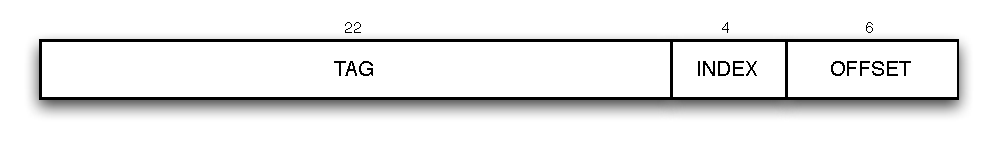
\includegraphics[scale=.9]{diagrammes/part-adresse}
	\end{figure}
\end{ques}

\begin{ques}
	Donner l'état de ce cache de données après le premier tour de boucle en remplissant le tableau ci-dessous. Le champ index contient l'index de la case du cache. Pour faciliter la compréhension, le champ étiquette contiendra l'adresse complète (sur 32 bits) du mot d'indice 0 de la ligne de cache concernée. Le champ data i contient le mot d'index i de la ligne de cache. On utilisera la notation hexadécimale, précédée de 0x pour les adresses et pour les données.
	
	\begin{tabularx}{\textwidth}{lllllXll}
		\toprule
		\emph{index} & \emph{valid} & \emph{tag} & \emph{data} 15 & \emph{data} 14 & $\cdots$ & \emph{data} 1 & \emph{data} 0\tabularnewline
		\midrule
		\midrule
		0 & 1 & 0x0004 & 0xF & 0xE & $\cdots$ & 0x1 & 0x0\tabularnewline
		\midrule
		4 & 1 & 0x0004 & 0x1E & 0x1C & $\cdots$ & 0x2 & 0x0\tabularnewline
		\midrule
		8 & 1 & 0x0004 & 0x10 & 0xF & $\cdots$ & 0x2 & 0x1\tabularnewline
		\bottomrule
	\end{tabularx}
	\begin{figure}[h]
		\center
		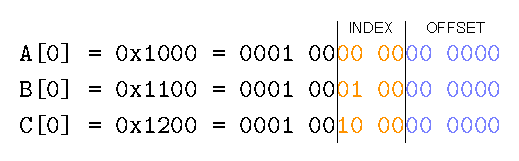
\includegraphics[scale=.9]{diagrammes/index-offset}
	\end{figure}
\end{ques}

\begin{ques}
	Nombre de MISS d-sur le cache de données pour les 3 premières itérations de la boucle : \begin{itemize}
		\item 1\iere itération : 3 MISS ;
		\item 2\ieme itération : 0 MISS ;
		\item 3\ieme itération : 0 MISS.
	\end{itemize}
	
	Sur les 64 itérations, il y a 4 MISS par tableau (0, 16, 32 et 48). Il y a donc $4\times 3$ MISS au total.
\end{ques}

\begin{ques}
	 La compilation de cette boucle génère une séquence de 20 instructions en assembleur MIPS 32 (on ne considère pas la déclaration des variables ni leur initialisation). Grâce à la technique de pipe-line, le CPI (nombre de cycle d'avec un système mémoire parfait est de 1 cycle par instruction. Le coût d'un MISS est de 10 cycles. On considère que le cache instruction se comporte comme un cache parfait (0 MISS).
	
	Temps total (en nombre de cycles horloge) nécessaire à l'exécution des 64 itérations de la boule.
	
	Il y a 20 instructions par itération, soit 20 cycles nécessaires pour exécuter une itération de la boucle.
	\[ T = 64\times 20+120 =  1400\;\mathrm{cycles}\]
	De ce fait, le CPI réel est égal à :\[CPI = \frac{64\times 20 + 120}{64\times 20} = 1,0938\]
\end{ques}

\clearpage

\section{Bus système} % (fold)

On considère l’architecture matérielle ALMO5 (utilisée en TP). Cette architecture contient un seul processeur (avec ses caches de 1\ier niveau), un timer, un terminal écran/clavier de type TTY, un contrôleur graphique (« frame buffer ») permettant d’afficher des images, une ROM contenant le « code de boot », un cache de 2\ieme niveau permettant d’accéder à la mémoire externe, et deux périphériques possédant une capacité d’adressage de la mémoire : le contrôleur DMA permet de transférer des données d’un tampon mémoire vers un autre. Le contrôleur I/O permet de transférer des données entre le disque et un tampon mémoire.

\begin{figure}[h]
	\center
	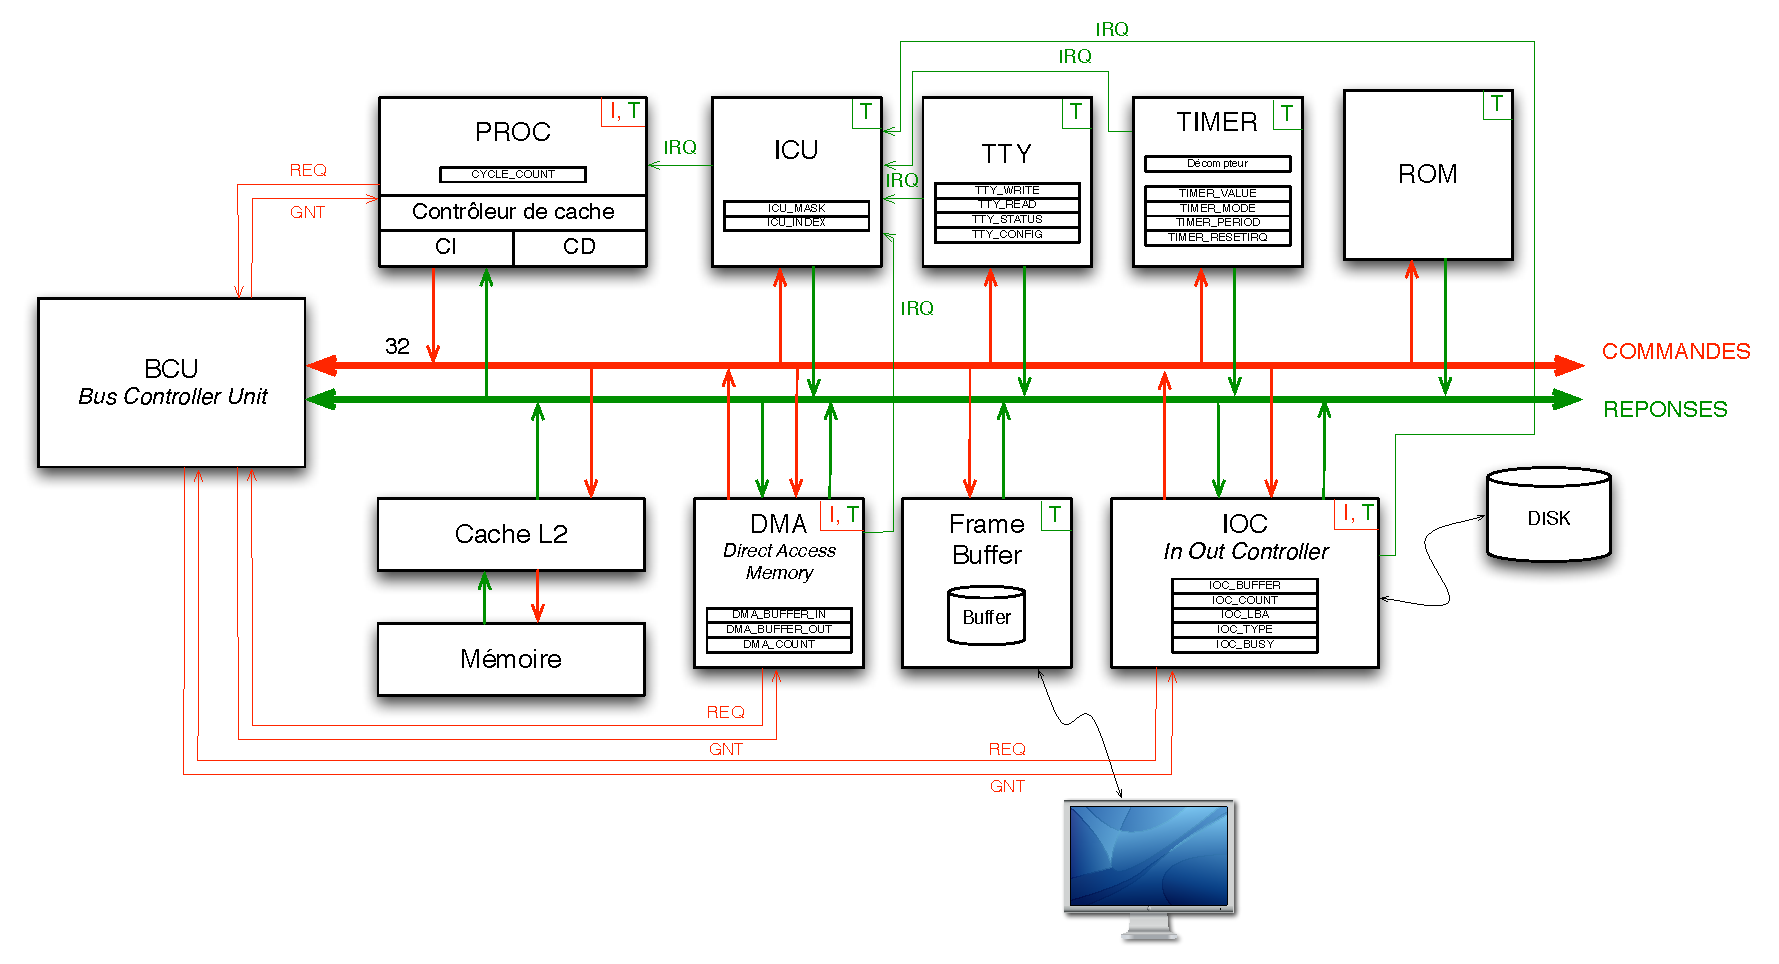
\includegraphics[scale=.5]{diagrammes/architecture-finale}
\end{figure}

On suppose que des images sont stockées sur le disque, et qu’on cherche à afficher une séquence d’image en respectant la cadence vidéo. La fréquence vidéo est de 25 images par seconde (une nouvelle image doit être affichée toutes les 40 ms). Comme dans le TP18, l’affichage d’une image nécessite trois étapes :\begin{itemize}
	\item \textbf{Phase Load} : chargement de l’image depuis le disque vers un premier tampon mémoire appelé \lstinline!buf_in!. Ce transfert est réalisé par le contrôleur I/O ;
	\item \textbf{Phase Modif} : le processeur lit l’image stockée dans \lstinline!buf_in!, la modifie, et recopie l’image modifiée dans un second tampon mémoire \lstinline!buf_out! ;
	\item \textbf{Phase Display} : affichage de l’image par copie du tampon \lstinline!buf_out! vers la mémoire vidéo. Ces transferts (lecture puis écriture) sont réalisés par le DMA.
\end{itemize}

Le but général de l'exercice est de déterminer la taille maximale d'une image, en faisant l'hypothèse que le facteur limitant est la bande passante du bus (mesurée en nombre d'octets par cycle). On suppose que l'image est codée en « niveaux de gris », et que chaque pixel est codé sur 8 bits. On notera $N$ le nombre total de pixels d'une image : Par exemple, une image de 400 lignes de 600 pixels a une taille de $N = 240\,000$ pixels.

On suppose que cette architecture est celle d'un système embarqué (tel qu'un téléphone mobile), qui fonctionne à 25 MHz. Cette fréquence est assez basse, pour limiter la consommation d'énergie, et augmenter la durée de vie de la batterie. La largeur du bus est de 32 bits, ce qui signifie qu'on peut transférer au plus un mot de 32 bits par cycle.


\begin{ques}
	Composant maître : composant capable de démarrer une transaction vers l'espace adressable. Il y a 3 composants maîtres : PROC, DMA, BLOCK I/O.
	
	Un composant cible est une composant qui termine la transaction en répondant à la commande. Il y a 8 composants cibles : ICU, TTY, TIMER, ROM, Cache L2, DMA, FB et BLOCK I/O.
	
	La cible d'une transaction est désignée / sélectionnée par les bits de poids fort de l'adresse (MSB) --- décodée par le BCU.
\end{ques}

\begin{ques}\label{ques:c2}
	Cette architecture fonctionner à une fréquence de 25 MHz. Il y a donc 25 millions de cycles par seconde.
	
	Puisqu'il y a 25 images par seconde, alors il y a 1 million de cycles entre deux affichages. 
	
	La bande passante maximale du bus est égale à 4 octets / cycles puisque la largeur du bus est de 32 bits ($=4$ octets).
	
	Pour transférer une image de $N$ pixels entre deux composants matériels, il faut alors $\nicefrac{N}{4}$ cycles.
\end{ques}

\begin{ques}
	Pour chaque image affichée, le nombre de transferts est :\begin{itemize}
		\item Phase load : 1 transfert ;
		\item Phase modif : 2 transferts ;
		\item Phase display : 2 transferts ;
	\end{itemize}
	
	Il y a donc 5 transferts par image. Il faut alors $T = 5\times \nicefrac{N}{4}$ cycles pour afficher une image.
	
	Or $N_{max} = T\times \nicefrac{4}{5} = 1\,000\,000\times\nicefrac{4}{5} = 600\,000$ pixels (cf question \ref{ques:c2} : il y a $T=1\,000\,000$ cycles entre deux affichages).
\end{ques}

\clearpage

\section{Interruptions et mémoire virtuelle} % (fold)

Cochez une seule réponse pour chaque question

\begin{ques}
	On considère la plateforme matérielle de l'exercice 3. Combien faut-il connecter d'entrées d'interruption au contrôleur d'interruptions (ICU) ?
\begin{description}
	\setlength{\itemsep}{2pt}
	\setlength{\parskip}{-1pt}
	\setlength{\parsep}{-1pt}
	\item[\Square] 3
	\item[\CheckedBox] 4 (TIMER, ICU, DMA, IOC)
	\item[\Square] 5
	\item[\Square] 8
\end{description}
\end{ques}

\begin{ques}
	Pour une certaine application logicielle, on ne souhaite utiliser que deux types d'interruptions : l'interruption du contrôleur I/O est connectée sur l'entrée 6 de lCU, et l' interruption du terminal écran/clavier est connectée sur l'entrée 2. Quelle valeur faut-il écrire dans le registre de masque de l'ICU pour n'autoriser que ces 2 interruptions ?
\begin{description}
	\setlength{\itemsep}{2pt}
	\setlength{\parskip}{-1pt}
	\setlength{\parsep}{-1pt}
	\item[\Square] 0x0100 0100
	\item[\CheckedBox] 0x0000 0044 (... 0100 0100)
	\item[\Square] 0x0000 0062
	\item[\Square] 0xFFFF FFFF
\end{description}
\end{ques}

\begin{ques}
	Une tâche s'exécutant sur le processeur est interrompue par une interruption. Donner la succession des événements qui se produisent dans le système (l'ordre est important).
\begin{description}
	\setlength{\itemsep}{2pt}
	\setlength{\parskip}{-1pt}
	\setlength{\parsep}{-1pt}
	\item[\Square] Acquittement interruption, Sauvegarde par le processeur du compteur ordinal dans EPC, Saut du processeur à l'adresse \lstinline!int_handler!, Saut du processeur à l'adresse 0x80000180
	\item[\Square] Saut du processeur à l'adresse 0x80000180, Sauvegarde par le processeur du compteur ordinal dans EPC, Saut du processeur à l'adresse \lstinline!int_handler!, Acquittement interruption
	\item[\Square] Saut du processeur à l'adresse \lstinline!int_handler!, Acquittement interruption, Sauvegarde par le processeur du compteur ordinal dans EPC, Saut du processeur à l'adresse 0x80000180
	\item[\CheckedBox] Sauvegarde par le processeur du compteur ordinal dans EPC, Saut du processeur à l'adresse 0x80000180, Saut du processeur à l'adresse \lstinline!int_handler!, Acquittement interruption
\end{description}
\end{ques}

\begin{ques}
	Que fait l'instruction \lstinline!eret! du processeur MIPS32 ?
\begin{description}
	\setlength{\itemsep}{2pt}
	\setlength{\parskip}{-1pt}
	\setlength{\parsep}{-1pt}
	\item[\Square] Elle branche à l'adresse contenue dans le registre \$31 et interdit les interruptions.
	\item[\Square] Elle branche à l'adresse contenue dans le registre \$31 et autorise les interruptions.
	\item[\Square] Elle branche à l'adresse contenue dans le registre EPC et interdit les interruptions.
	\item[\CheckedBox] Elle branche à l'adresse contenue dans le registre EPC et autorise les interruptions.
\end{description}
\end{ques}

\begin{ques}
	Pourquoi les registres \$26 et \$27 du processeur ne doivent pas être utilisés par un programme utilisateur ?
\begin{description}
	\setlength{\itemsep}{2pt}
	\setlength{\parskip}{-1pt}
	\setlength{\parsep}{-1pt}
	\item[\Square] Ces registres sont protégés. Un accès illégal à ces registres en mode utilisateur déclenche un départ en exception.
	\item[\Square] Ces registres sont réservés au système d'exploitation et contiennent des informations importantes du système d'exploitation qui ne doivent pas être connues des utilisateurs.
	\item[\CheckedBox] ECes registres sont utilisés par le gestionnaire d'interruption, exceptions et trappes, et peuvent donc être modifiés à tout moment en cas d'interruption.
\end{description}
\end{ques}

\begin{ques}
	Dans un système de mémoire virtuelle paginée, la MMU (\emph{Memory Management Unit}) utilise des tables de pages indexées par le numéro de page virtuelle pour définir la correspondance entre les adresses virtuelles et les adresses physiques.
\begin{description}
	\setlength{\itemsep}{2pt}
	\setlength{\parskip}{-1pt}
	\setlength{\parsep}{-1pt}
	\item[\Square] La table de page est construite par le système d'exploitation et cette unique table est utilisée par tous les programmes des utilisateurs.
	\item[\Square] Chaque programme utilisateur construit et utilise sa propre table de page.
	\item[\CheckedBox] La table de page d'un programme utilisateur est construite par le système d'exploitation, et il y a autant de tables de pages que de programmes utilisateurs.
\end{description}
\end{ques}

\begin{ques}
	Pourquoi les tables de pages ont-elles souvent une organisation à plusieurs niveaux ?
\begin{description}
	\setlength{\itemsep}{2pt}
	\setlength{\parskip}{-1pt}
	\setlength{\parsep}{-1pt}
	\item[\Square] Une table de page à 2 niveaux se parcourt plus rapidement qu'une table de pages à 1 niveau et occupe moins de place en mémoire qu'une table de page à 1 niveau.
	\item[\Square] Une table de pages à 2 niveaux se parcourt plus rapidement qu'une table de pages à 1 niveau mais occupe plus de place en mémoire qu'une table de page à 1 niveau.
	\item[\CheckedBox] Une table de page à 2 niveaux se parcourt moins rapidement qu'une table de pages à 1 niveau mais occupe moins de place en mémoire qu'une table de page à 1 niveau.
\end{description}
\end{ques}

\begin{ques}
	La TLB (\emph{Translation Look-aside Buffer}) est un petit cache contenant les plus récentes traductions (VPN $\Leftrightarrow$ PPN). Que se passe-t-il (dans le cas général) en cas de MISS sur la TLB ?
\begin{description}
	\setlength{\itemsep}{2pt}
	\setlength{\parskip}{-1pt}
	\setlength{\parsep}{-1pt}
	\item[\Square] Le processeur est gelé pendant 10 cycles en attendant que la MMU aille rechercher la traduction (VPN $\Leftrightarrow$ PPN) manquante en mémoire, puis le programme reprend son exécution.
	\item[\CheckedBox] Le processeur est gelé pendant une centaine de cycles, car la MMU doit faire plusieurs accès à la mémoire pour parcourir les tables de pages, puis le programme reprend son exécution.
	\item[\Square] Le programme qui a fait un MISS TLB est systématiquement interrompu, et le système d'exploitation attribue le processeur à un autre programme, car un défaut de page nécessite un accès au disque, qui coûte plusieurs centaines de milliers de cycles.
\end{description}
\end{ques}

\begin{ques}
	Lors d'une commutation de tâches dans un système possédant un mécanisme de mémoire virtuelle,
\begin{description}
	\setlength{\itemsep}{2pt}
	\setlength{\parskip}{-1pt}
	\setlength{\parsep}{-1pt}
	\item[\Square] Le système ne s'occupe pas de la MMU.
	\item[\Square] Le système doit modifier le registre PTPR contenant l'adresse de base de la table des pages.
	\item[\Square] Le système se contente d'invalider les entrées « utilisateur » de la TLB.
	\item[\CheckedBox] le système modifie le registre PTPR et invalide les entrées « utilisateur » de la TLB.
\end{description}
\end{ques}

\begin{ques}
	Le fichier ldscript (étudié en TD et TP) contient les directives de regroupement des différentes sections dans différents segments, et définit les adresses de base de ces segments mémoire.
\begin{description}
	\setlength{\itemsep}{2pt}
	\setlength{\parskip}{-1pt}
	\setlength{\parsep}{-1pt}
	\item[\Square] Il est utilisé par l'éditeur de liens et définit des adresses physiques.
	\item[\CheckedBox] Il est utilisé par l'éditeur de liens et définit des adresses virtuelles.
	\item[\Square] Il est utilisé pour générer les fichiers \lstinline!.o! et définit des adresses physiques.
	\item[\Square] Il est utilisé pour générer les fichiers \lstinline!.o! et définit des adresses virtuelles.
\end{description}
\end{ques}

\end{document}